\documentclass{beamer}
\usetheme{Boadilla}
\usecolortheme{crane}
\usefonttheme[stillsansseriflarge, stillsansserifsmall]{serif}
%\usefonttheme[stillsansseriflarge, stillsansserifsmall]{structurebold}
%\usefonttheme[onlymath]{serif}
\useinnertheme{default}
\setbeamertemplate{navigation symbols}{}

\usepackage{fontspec}
%\usepackage{kpfonts}
\setmainfont[Numbers=OldStyle]{Tex Gyre Pagella}
\setsansfont[BoldFont=Lovelo-LineBold]{Lovelo-LineBold}

\usepackage[frenchb]{babel}


%proper math and math symbols
%\usepackage{amsmath}
\usepackage{amssymb}

\usepackage{siunitx}
\sisetup{
  mathsmu = \text{µ},
  textmu  = µ
}
\usepackage{booktabs}
\usepackage{multirow}

% Allow the usage of graphics (.jpg, .png, etc.) in the document
\usepackage{graphicx}

\usepackage{tikz}
\usetikzlibrary{calc, positioning, intersections, matrix, patterns}
\usepackage{pgfplots}
\usepgfplotslibrary{groupplots}

\pgfplotsset{compat=1.3, every axis/.append style={mark size={0.2em}}}

\usepgfplotslibrary{external}
\tikzset{external/system call={lualatex \tikzexternalcheckshellescape -halt-on-error -interaction=batchmode -jobname "\image" "\texsource"}}


\definecolor{Main}{rgb}{1, 0.57, 0}
\definecolor{Accent1}{rgb}{1,0.28,0}
\definecolor{Accent2}{rgb}{1,0.74,0}


%\tikzexternalize

\usepackage{multimedia}

%bibliography
\usepackage{natbib}
%\usepackage{bibentry}
\def\newblock{\hskip .11em plus .33em minus .07em}

\institute{ENS Lyon}
\title{Yaourt pliss\'{e}, yaourt flamb\'{e}}

\author[M. Leocmach]{Mathieu Leocmach}
\date{13 Novembre 2013}

\begin{document}
\tikzset{every mark/.append style={scale=0.8}}
\pgfplotsset{every axis/.append style={small}}
\tikzset{external/force remake=false}

\AtBeginSection[]{
	\addtocounter{framenumber}{-1}
	\begin{frame}[plain]
		\tableofcontents[currentsection, hideothersubsections]
	\end{frame}
}

\begin{frame}[plain]
	\titlepage
\end{frame}

\begin{frame}{Motifs}
	\begin{tikzpicture}[inner sep=0, very thick]
	\node[anchor=west] (a) {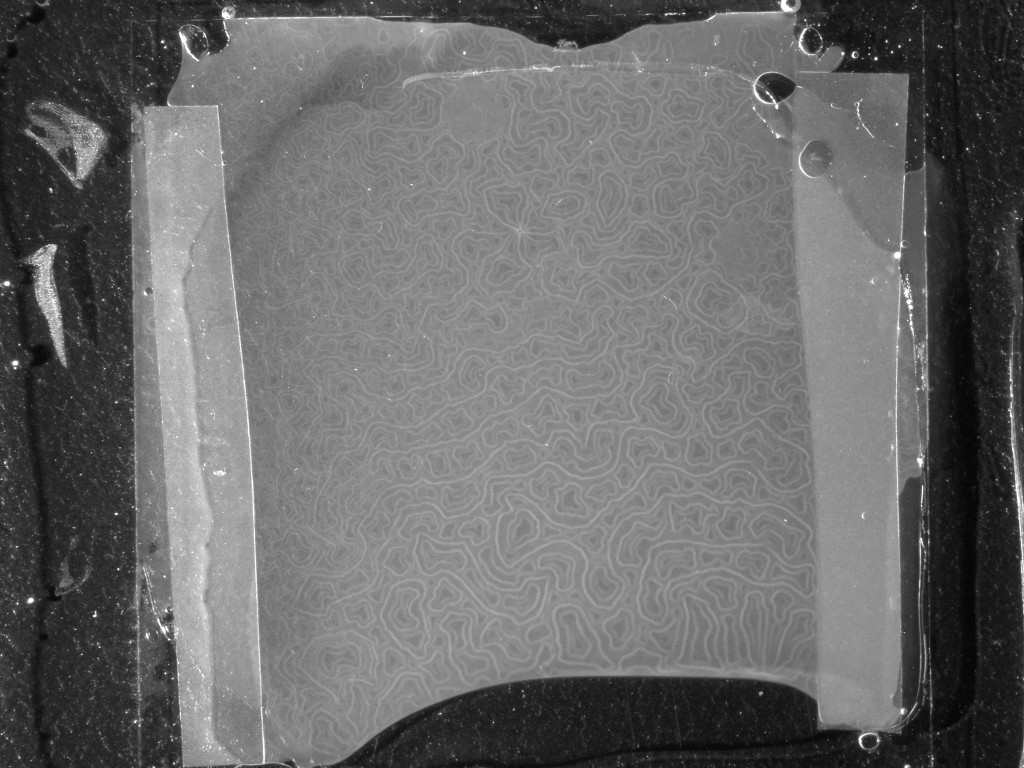
\includegraphics[width=0.3\columnwidth]{cas3p2_fluo0p8_GDL4_50um_coating_2_zoom2}};
		\node at (0.5\columnwidth,0) (b) {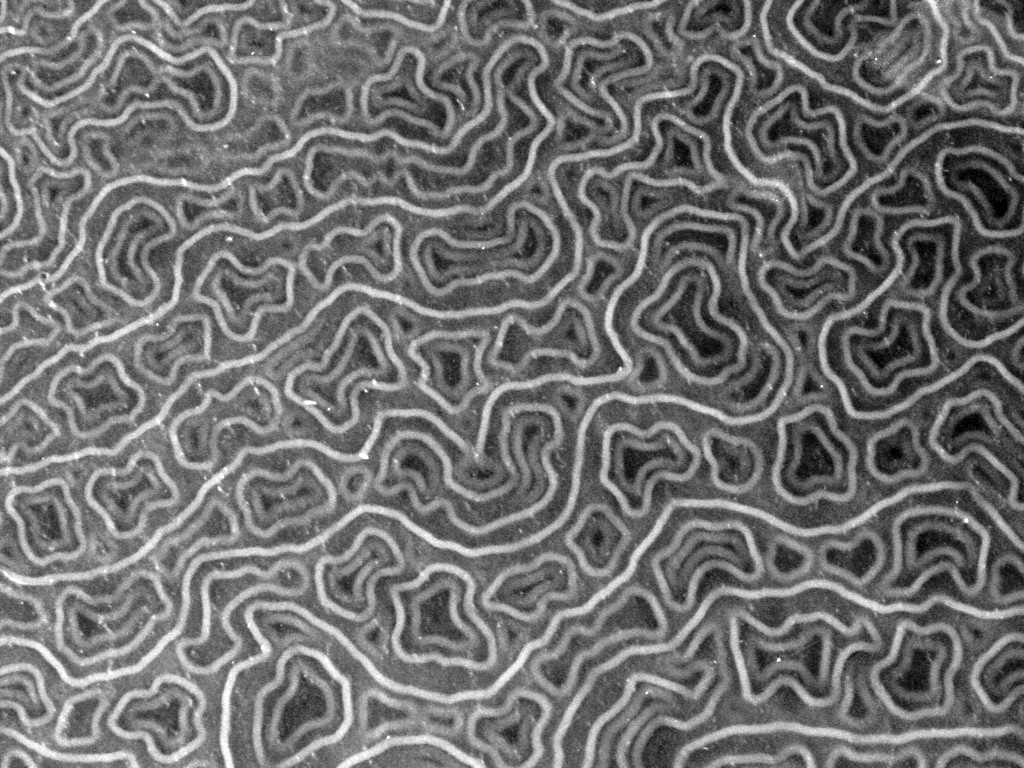
\includegraphics[width=0.3\columnwidth]{cas3p2_fluo0p8_GDL4_50um_coating_2_zoom6}};
		\node[anchor=east] at (\columnwidth,0) (c) {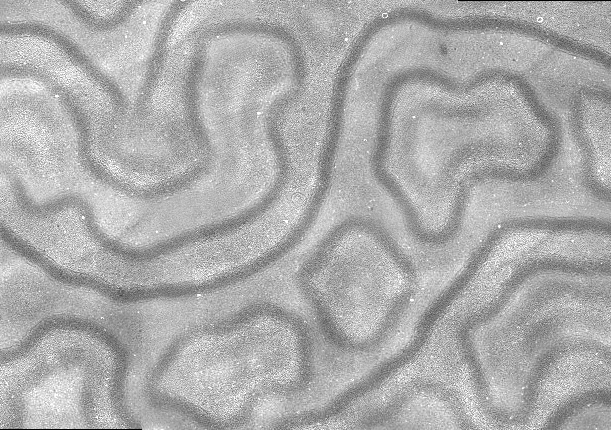
\includegraphics[width=0.3\columnwidth]{cas3p2_fluo0p8_GDL4_50um_coating_2_transmission}};
		\draw[Accent2] (a.north west) ++(0.126\columnwidth, -0.086\columnwidth) rectangle +(0.1\columnwidth,-0.075\columnwidth) -- (b.south west) (a.north west) ++(0.226\columnwidth, -0.086\columnwidth) -- (b.north west) rectangle (b.south east);
		\draw[Main] (b.north west) ++(0.117\columnwidth,-0.117\columnwidth) rectangle +(0.093\columnwidth,-0.068\columnwidth) -- (c.south west) (b.north west) ++(0.211\columnwidth,-0.117\columnwidth) --(c.north west) rectangle (c.south east);
		\draw[Accent1] (c.north west) ++(0.094\columnwidth,0) rectangle +(0.117\columnwidth,-0.117\columnwidth);
		\draw[ultra thick] (a.south east) ++(0,-0.25em) -- ++(-0.106\columnwidth,0) node[pos=0.5, below=0.25em, font=\small] (M) {\SI{1}{\centi\metre}};
		\draw[ultra thick] (b.south east) ++(0,-0.25em) -- ++(-0.158\columnwidth,0) node[pos=0.5, below=0.25em, font=\small] {\SI{5}{\milli\metre}};
		\draw[ultra thick] (c.south east) ++(0,-0.25em) -- ++(-0.099\columnwidth,0) node[pos=0.5, below=0.25em, font=\small] {\SI{1}{\milli\metre}};
		\node[above=0 of a] {Reflexion Macroscope};
		\node[above=0 of b] {Reflexion Macroscope};
		\node[above=0 of c, text width=0.3\columnwidth] {Transmission\linebreak Microscope (tiled)};
	\end{tikzpicture}
\end{frame}

\begin{frame}{Acid-induced gels}
	
	In millipore water
	\begin{itemize}
	\item 4\% Sodium caseinate (milk protein)\hfill
	Isoelectric point $\approx 4.6$
	\item 4\% $\delta$-gluconolactone (\textsc{gdl})\hfill
	Slow hydrolysis into gluconic acid
	\end{itemize}
	\vfill
	\begin{tikzpicture}
	\begin{groupplot}[%
		group style={
			group size=1 by 2, 
			xlabels at=edge bottom, 
			xticklabels at=edge bottom,
			vertical sep=1em,
			},
		xmin=0, xmax=8,
		xlabel={time (h)}, 
		extra tick style={grid=major},%
		extra y ticks={4.6}, extra y tick labels={},%
		extra x ticks={0.55, 0.64, 0.72, 0.80, 1, 1.27, 2.5}, extra x tick labels={},%
		width=\columnwidth,
		height=0.25\columnwidth,
		]
	\nextgroupplot[ylabel=pH, ymin=0, ymax=7]
	\addplot+[no marks,Accent1] table[x expr={\thisrowno{0}/3600.+0.05}]{Y189_28800s.pH};
	\node[base left] at (axis cs:8,4.6) {isoelectric};
	\nextgroupplot[ylabel=$G^\prime$ (\si{\pascal}), ymin=0]
	\addplot+[no marks,Accent2] table[x expr={\thisrowno{0}/3600.+0.05}]{Y235_28800s.prise};
	\end{groupplot}
	\end{tikzpicture}
\end{frame}


\begin{frame}{Cellule de microscopie}
\begin{center}
\begin{tikzpicture}
\fill[pattern=north east lines,pattern color=Accent2] (0,0) rectangle (\columnwidth,1.5em) node[midway,fill=white,inner sep=1pt] {glass};
		\fill[pattern=north east lines,pattern color=Accent2] (0,-2.5em) rectangle (\columnwidth,-4em) node[midway,fill=white,inner sep=1pt] {glass};
		\draw[line width=2pt,Accent1] (0.05\columnwidth,-2.5em) -- (0.95\columnwidth,-2.5em) (0.05\columnwidth,-1pt) -- (0.95\columnwidth,-1pt) node[pos=0, below right, inner sep=1pt, text width=0.5\columnwidth] {acrylamide brush ($10\sim \SI{100}{\nano\metre}$)};
		\fill[gray] (0,0) rectangle (0.05\columnwidth,-2.5em) (\columnwidth,0) rectangle (0.95\columnwidth,-2.5em) node[pos=1, above left] {spacer};
		\draw[<->] (0.75\columnwidth,-2pt) -- (0.75\columnwidth,-2.5em) node[midway,left] {$e\sim \SI{100}{\micro\metre}$};
		\draw[<->] (0.05\columnwidth,-4.25em) -- (0.95\columnwidth,-4.25em) node[midway,below] (L) {$L\sim\SI{2}{\centi\metre}$};
\end{tikzpicture}
\end{center}

\begin{itemize}
\item Pas d'accroche sur les plus grandes surfaces grâce aux brosses.
\item Accroche sur les extrémités (spacers solides, pas d'interface libre)
\item Pas de contrainte extérieure
\end{itemize}
\end{frame}



\begin{frame}{Formation}
\begin{columns}
\column{0.5\textwidth}
\movie[externalviewer]{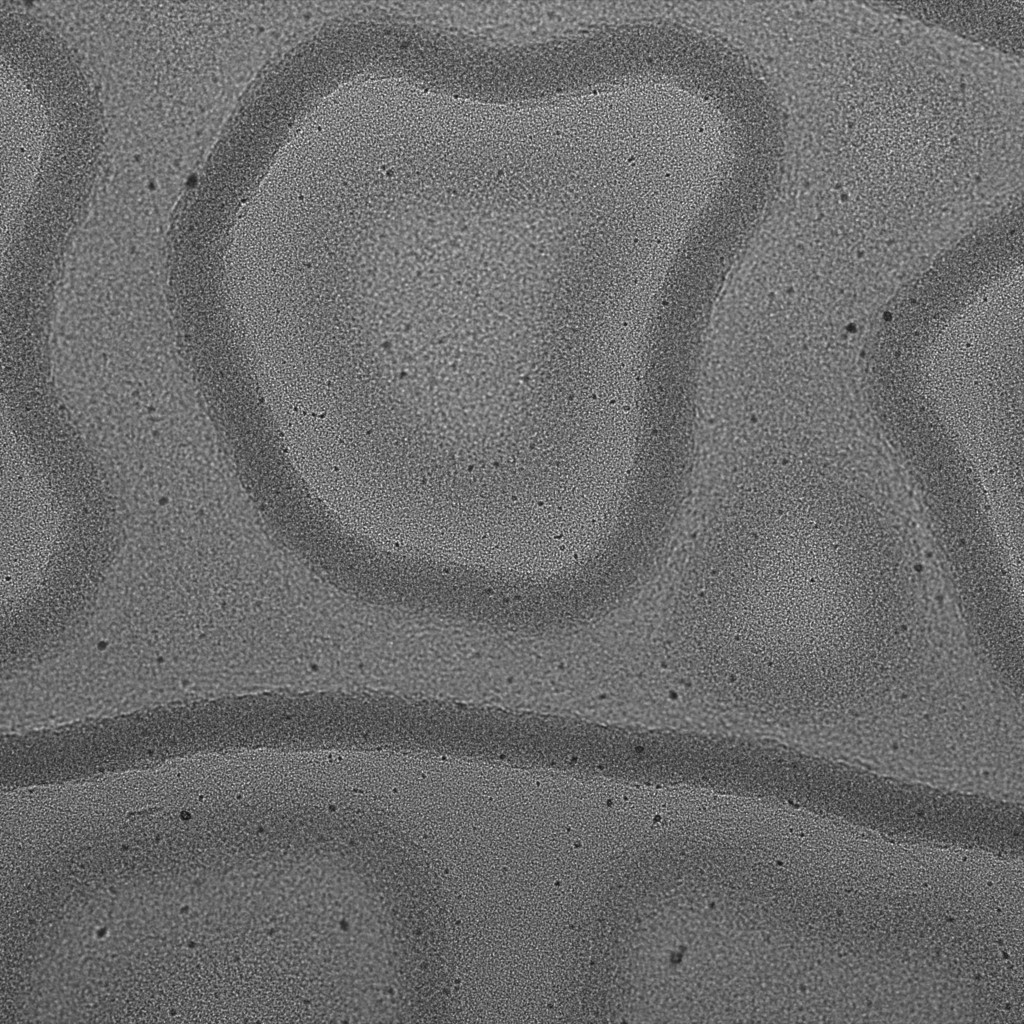
\includegraphics[width=\textwidth]{cas4_GDL4_motif_final.jpg}}{cas4_GDL_4_100um_coat_1_1_comp_4.avi}\\
\begin{tikzpicture}
\draw[ultra thick](0,0)-- (0.757\textwidth,0) node[midway, below] {\SI{1}{\milli\metre}};
\end{tikzpicture}
\column{0.5\textwidth}
\movie[externalviewer]{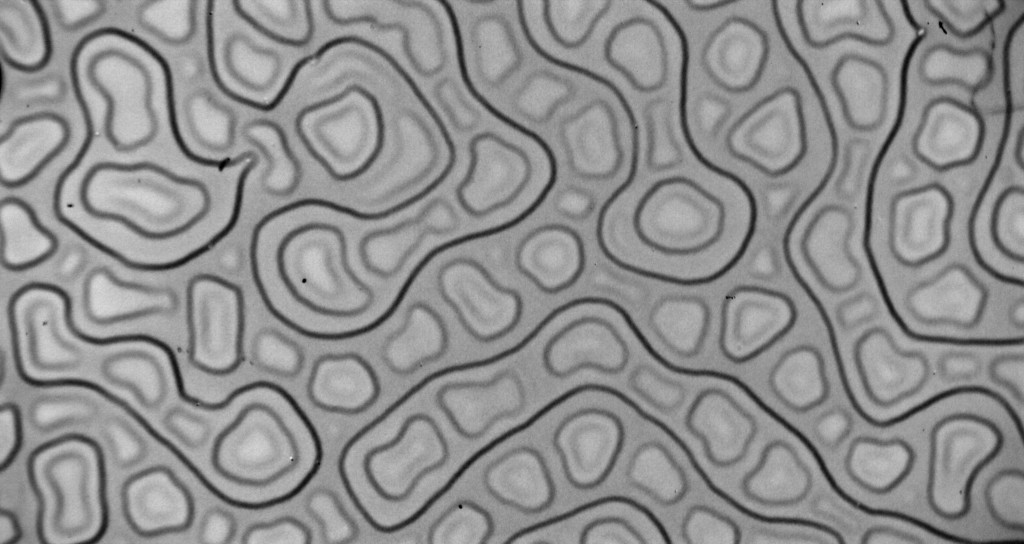
\includegraphics[width=\textwidth]{pattern_100um.jpg}}{cas4_GDL_4_100um_coat_macroscope_2.avi}\\
\begin{tikzpicture}
\draw[ultra thick](0,0)-- (0.177\textwidth,0) node[midway, below] {\SI{1}{\milli\metre}};
\end{tikzpicture}
\end{columns}
\end{frame}

\begin{frame}{Formation}
	\begin{tikzpicture}
	\matrix[matrix of nodes, inner sep=0, column sep=0.015\textwidth, row sep=0.5em, ampersand replacement=\&] (m){
	33 min \& 38 min \& 43 min \\
	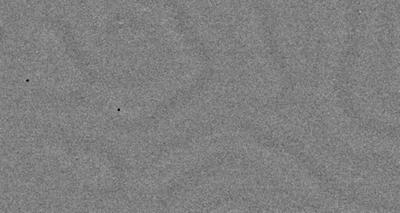
\includegraphics[width=0.32\textwidth]{prise_0100_resized.jpg}\&
	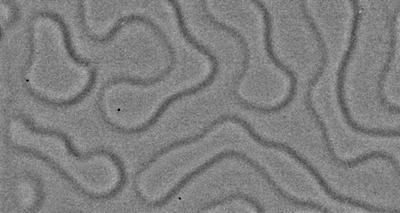
\includegraphics[width=0.32\textwidth]{prise_0130_resized.jpg}\&
	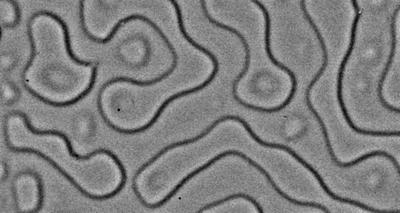
\includegraphics[width=0.32\textwidth]{prise_0160_resized.jpg}\\
	48 min \& 1h \& 1h15\\
	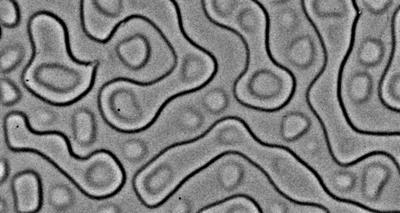
\includegraphics[width=0.32\textwidth]{prise_0190_resized.jpg}\&
	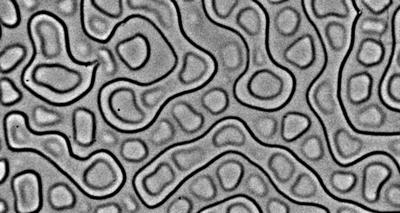
\includegraphics[width=0.32\textwidth]{prise_0250_resized.jpg}\&
	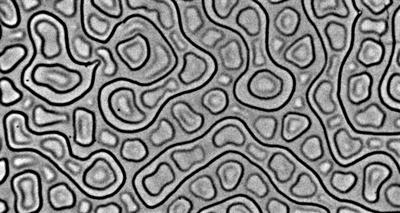
\includegraphics[width=0.32\textwidth]{prise_0360_resized.jpg}\\
	};
	\draw[ultra thick] ++(m-2-1.south west) -- ++(0.059\textwidth,0);
	\end{tikzpicture}
\end{frame}


\begin{frame}{Microscopie confocale}
%\begin{columns}
%\column{0.5\textwidth}
	\begin{block}{Procedure}
	\begin{itemize}
		\item Fluorescently label 10\% of the casein
		\item A confocal slice every \SI{5}{\micro\metre}
		\item $(\SI{1.3}{\milli\metre})^2 \times \SI{120}{\micro\metre}$
		\hfill $\Rightarrow$ Protein density field
		\item Detect top and bottom surfaces of the gel phase
	\end{itemize}
	\end{block}
%\column{0.5\textwidth}
\begin{center}
	\begin{tikzpicture}[inner sep=0]
		\node[above right]{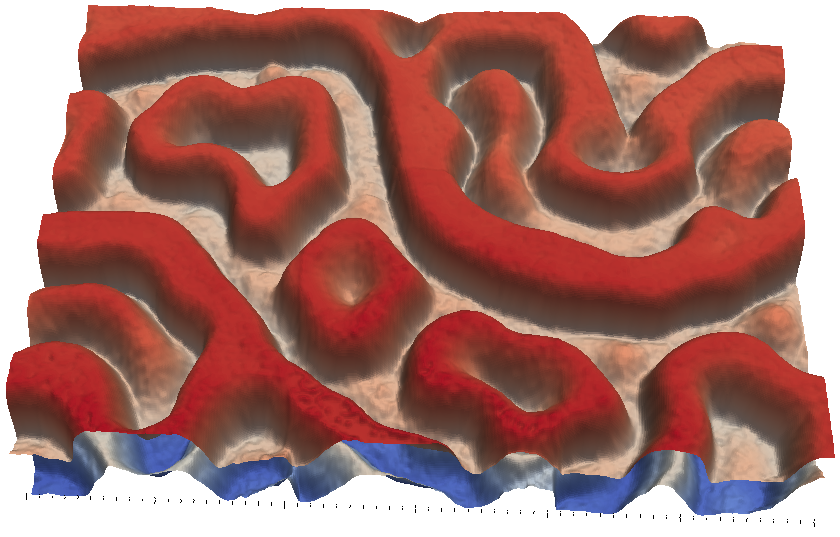
\includegraphics[width=0.6\textwidth]{collage_cut}};
		\draw[ultra thick] ++(0,0.5em) -- ++(0.2\textwidth,0) node[pos=0.5, below=0.25em, font=\small] {\SI{1}{\milli\metre}};
	\end{tikzpicture}
\end{center}
%\end{columns}
\end{frame}

\begin{frame}{Dynamique en confocal}
\begin{columns}
\column{0.5\textwidth}
\movie[externalviewer]{\includegraphics[width=\textwidth]{plots_final.jpg}}{plots.avi}
\column{0.5\textwidth}
\movie[externalviewer]{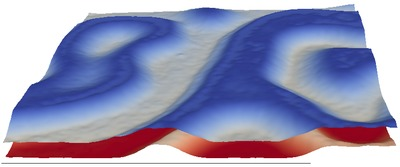
\includegraphics[width=\textwidth]{cas3p2_fluo0p8_GDL4_2_t260_crop_resized.jpg}}{paraview_cas3p3_fluo0p8_GDL4_2_flat2_comp.avi}
\end{columns}
\begin{tikzpicture}
	\begin{groupplot}[%
		group style={group name=g, group size=1 by 2},
		xmin=0, xtick={20,40,...,160},
		xlabel={time (min)}, 
		extra tick style={grid=major},%
		extra x ticks={33, 38, 43, 48, 58, 77, 150}, extra x tick labels={},%
		width=\columnwidth,
		height=0.25\columnwidth,
		]
	\nextgroupplot[ylabel={$V_\text{gel}/V_\text{cell}$}, ymin=0.5, ymax=1]
	\addplot+[no marks,Accent1] table[x expr={\thisrowno{0}/60.+3}]{cas4_GDL4_fluo0p4_2.volume};
	
	\nextgroupplot[ylabel={$A/A_\text{cell}-1$ (\%)}, ymin=0, ymax=2]
	\addplot+[no marks,Accent1] table[x expr={\thisrowno{0}/60.+3}]{cas4_GDL4_fluo0p4_2.area};
	\end{groupplot}
\end{tikzpicture}
\end{frame}

\begin{frame}{Dynamique}
\begin{tikzpicture}
	\matrix[
		matrix of nodes, inner sep=0, 
		column sep=0.015\textwidth, row sep=0.5em,
		ampersand replacement=\&] (m){
	33 min \& 38 min \& 43 min \& 48 min \& 1h \& 1h15 \& 2h30\\
	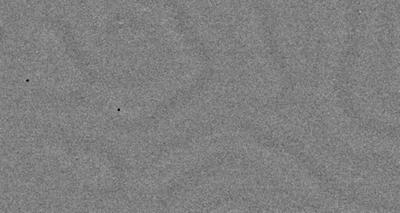
\includegraphics[width=0.13\textwidth]{prise_0100_resized.jpg}\&
	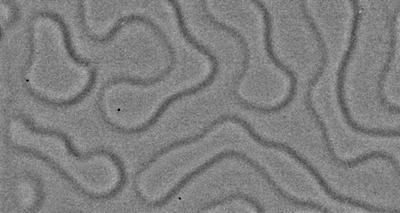
\includegraphics[width=0.13\textwidth]{prise_0130_resized.jpg}\&
	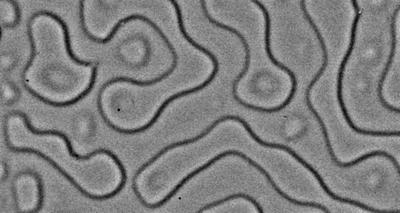
\includegraphics[width=0.13\textwidth]{prise_0160_resized.jpg}\&
	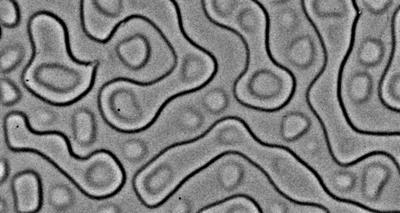
\includegraphics[width=0.13\textwidth]{prise_0190_resized.jpg}\&
	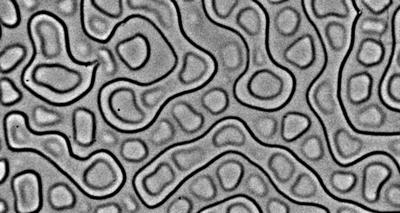
\includegraphics[width=0.13\textwidth]{prise_0250_resized.jpg}\&
	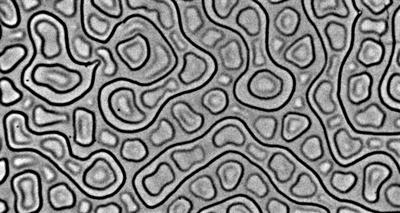
\includegraphics[width=0.13\textwidth]{prise_0360_resized.jpg}\&
	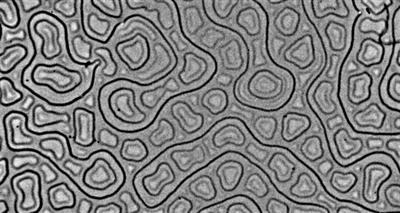
\includegraphics[width=0.13\textwidth]{prise_0799_resized.jpg}\\
	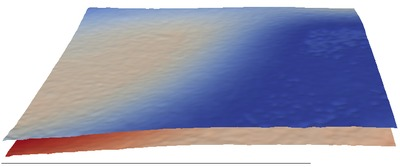
\includegraphics[width=0.13\textwidth]{cas3p2_fluo0p8_GDL4_2_t047_crop_resized.jpg}\&
	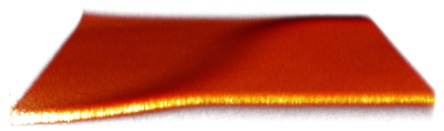
\includegraphics[width=0.13\textwidth]{cas3p2_fluo0p8_GDL4_2_t056_crop_resized.jpg}\&
	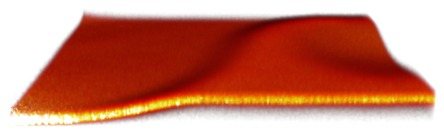
\includegraphics[width=0.13\textwidth]{cas3p2_fluo0p8_GDL4_2_t065_crop_resized.jpg}\&
	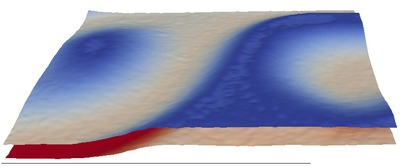
\includegraphics[width=0.13\textwidth]{cas3p2_fluo0p8_GDL4_2_t074_crop_resized.jpg}\&
	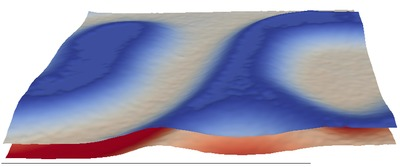
\includegraphics[width=0.13\textwidth]{cas3p2_fluo0p8_GDL4_2_t092_crop_resized.jpg}\&
	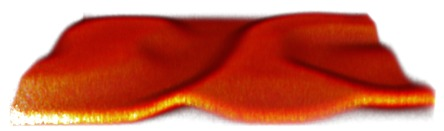
\includegraphics[width=0.13\textwidth]{cas3p2_fluo0p8_GDL4_2_t125_crop_resized.jpg}\&
	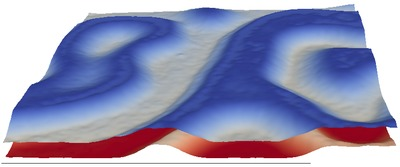
\includegraphics[width=0.13\textwidth]{cas3p2_fluo0p8_GDL4_2_t260_crop_resized.jpg}\\
	};
	\draw[ultra thick] ++(m-2-1.south west) -- ++(0.023\textwidth,0);
	\draw[ultra thick] ++(m-3-1.south west) -- ++(0.1\textwidth,0);
\end{tikzpicture}
\begin{columns}[T]
\column{0.29\textwidth}
\hrulefill\\
Motif primaire
\begin{itemize}
\item Parfois labyrinthe, parfois plots
\item Du sol au plafond
\end{itemize}
Rides sans substrat ?
\column{0.7\textwidth}
\hrulefill\\
Flambage $\Rightarrow$ harmoniques

\includegraphics[width=\columnwidth]{Roman_nouveau_plis.jpg}

Roman \& Pocheau, EPL (1999).
\end{columns}
\end{frame}

\begin{frame}{Longueurs d'onde en fonction du gap}
	\begin{tikzpicture}
	\matrix[
		matrix of nodes, inner sep=0, matrix anchor=south east, 
		column sep=0.033\columnwidth, row sep=0.5em,
		ampersand replacement=\&
		] (m) {
		\SI{50}{\micro\metre} \& \SI{100}{\micro\metre}\\
		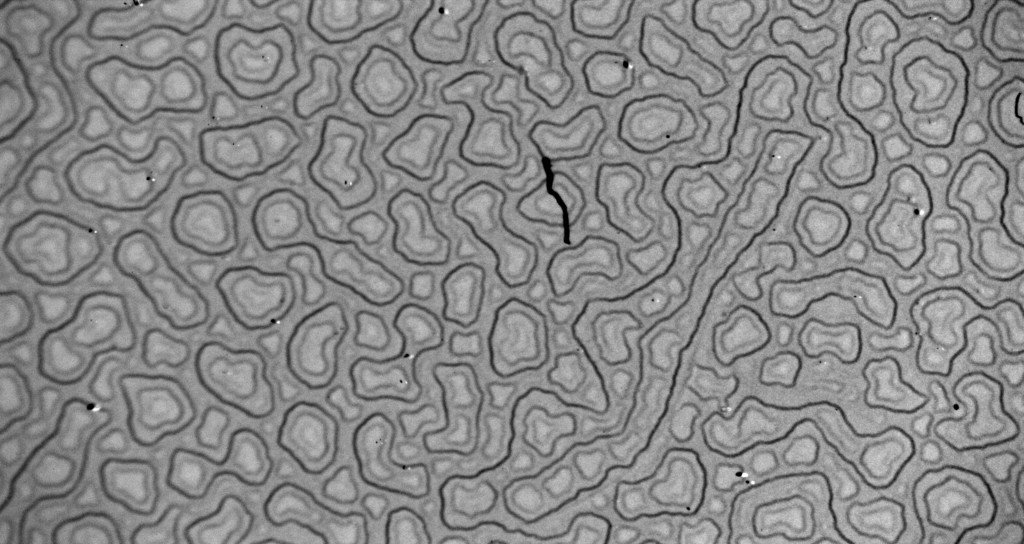
\includegraphics[width=0.225\columnwidth]{pattern_50um.jpg} \&
		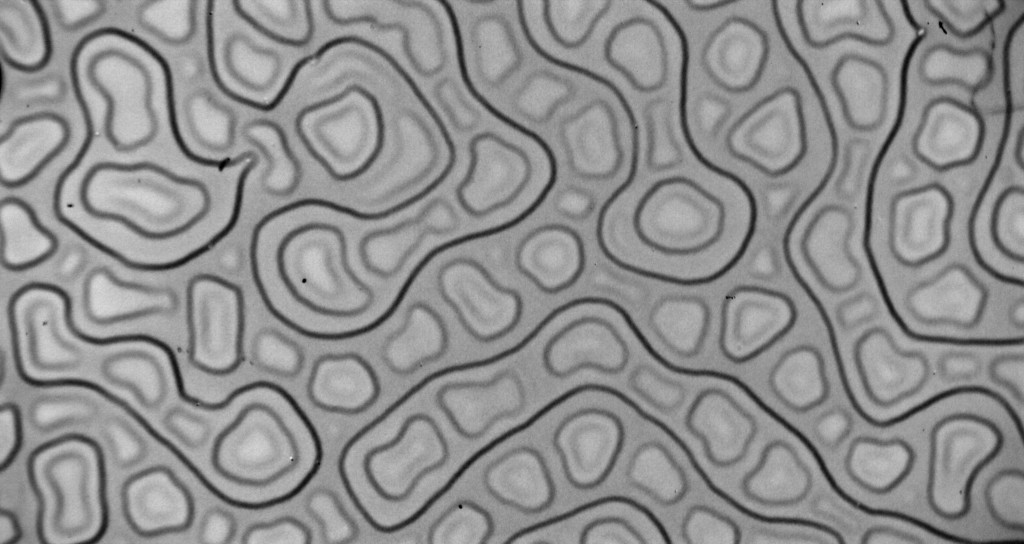
\includegraphics[width=0.225\columnwidth]{pattern_100um.jpg}\\
		\SI{250}{\micro\metre} \& \SI{450}{\micro\metre}\\
		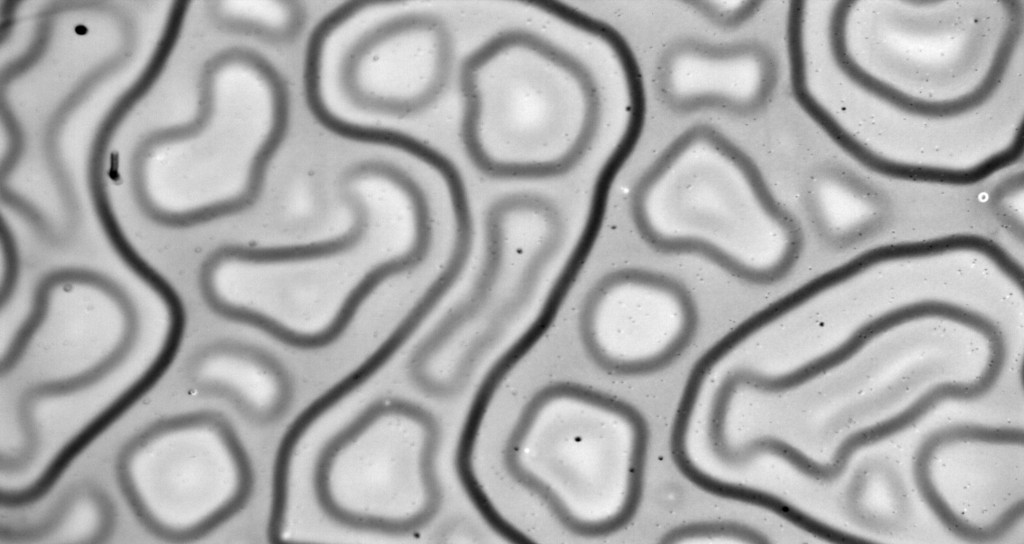
\includegraphics[width=0.225\columnwidth]{pattern_250um.jpg} \&
		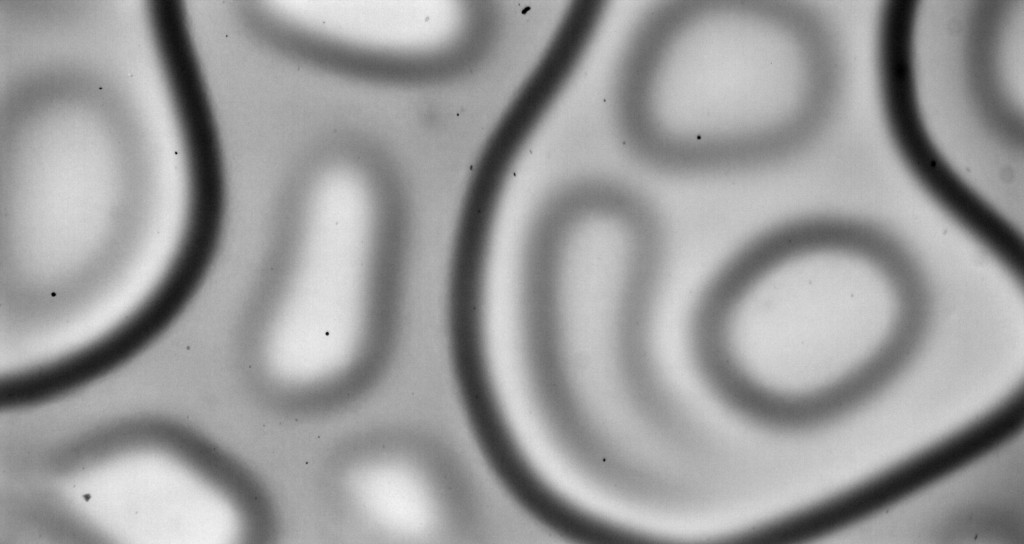
\includegraphics[width=0.225\columnwidth]{pattern_450um.jpg}\\
	};
	\node[inner sep=0, below=1.5em of m] (x800) {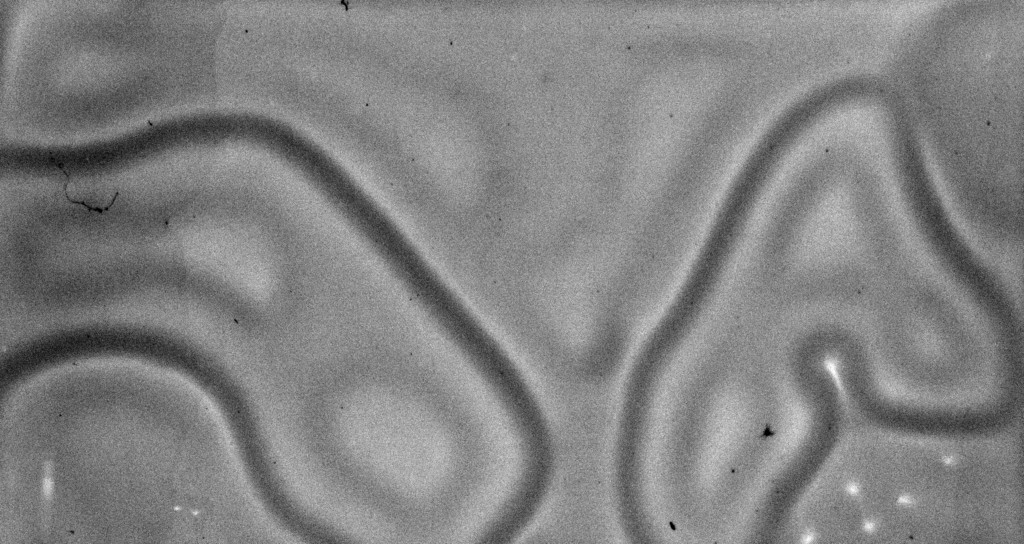
\includegraphics[width=0.45\columnwidth]{pattern_800um_x1.jpg}};
	\node[above = 0 of x800.north] {\SI{800}{\micro\metre}};
	\draw[ultra thick, Accent2, <->] (x800.south west) ++(0.18\columnwidth, 0.05\columnwidth) -- ++(0.133\columnwidth,0) node[midway,above]{$\lambda$};
	\draw[ultra thick](x800.north east) ++(0,-0.5em) -- ++(-0.2\columnwidth,0) node[midway, below] {\SI{5}{\milli\metre}};
	\begin{axis}[%
		name=g,
		at={($(m-2-1.west)+(\columnwidth,0)$)},
		anchor=outer north east,
		width=0.5\columnwidth,
		height=0.5\columnwidth,
		xmin=0,xmax=1,xlabel={gap (\si{\milli\metre})},
		xtick={0.1,0.3,...,0.9},
		ymin=0, ymax=4.23, ylabel={$\lambda$ (\si{\milli\metre})},
		]
		\addplot+[only marks,Accent1, mark options={fill=Accent1}] coordinates {(0.05,0.261) (0.1,0.458) (0.250,0.916) (0.450,2.075) (0.800,3.333)};
		\addplot+[domain=0:3, no marks, Accent1, forget plot] {4.23*x};
	\end{axis}
	\node[anchor=base west] at (x800.south east) {Longueur d'onde du motif primaire};
	\node [above = 0 of g] {$\lambda = 4.23 e$};
	\end{tikzpicture}
\end{frame}

\begin{frame}{Motif primaire: modèle}
Comment plisser (et non flamber) sans substrat ?
\begin{itemize}
\item Notre substrat, c'est l'eau
\hfill {\footnotesize Boudaoud \& Chaïeb, PRE (2001)}
\begin{itemize}
\item $E_s = \frac{3\eta}{\tau}$\qquad avec $\tau$ le temps caractéristique de l'écoulement
\item Epaisseur du substrat $H = \frac{e-h}{2} \approx e/4$. Substrat fin $H<\lambda$.
\end{itemize}
\item Pour un substrat d'un seul côté \hfill{\footnotesize Cerda \& Mahadevan, PRL (2003)} 
\end{itemize}
\begin{columns}
\column{0.6\textwidth}
\[
\lambda = \underbrace{\sqrt{hH}}_{\lessapprox 0.35e} \left(\underbrace{\frac{E_f}{E_s}}_{\approx 87\cdot 10^6}\right)^\frac{1}{6}
\approx 7.4e
\]
\column{0.4\textwidth}
\begin{align*}
G^\prime_f &\approx \SI{500}{\pascal}\Rightarrow
E_f \approx \SI{1300}{\pascal}\\
\tau &\approx \SI{200}{\second}\\
\eta &\approx \SI{1}{\milli\pascal\second}
\end{align*}
\end{columns}
\vfill
\begin{itemize}
\item Amplitude maximum contrainte $A=e-h\approx h\Rightarrow U_B \approx U_S$ \item Parfois rides parfois plots 
\hfill {\footnotesize Vandeparre \textit{et al.}, Soft Matter (2011)}
\end{itemize}
\end{frame}


\begin{frame}{Longueurs d'onde et composition}
\begin{columns}[T]\small

\column{0.45\textwidth}
\begin{block}{Moins de GDL}
\begin{itemize}
		\item Cinétique lente
		\item Gel plus fort
		\item Moins d'overshoot
	\end{itemize}
\end{block}
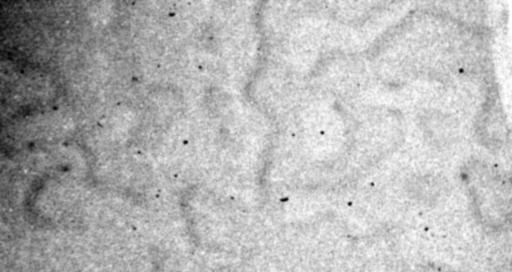
\includegraphics[width=0.75\textwidth]{cas4_GDL1.jpg}1\%
\begin{itemize}
\item Motif primaire uniquement 
\item Même longueur d'onde
\item Difficile d'obtenir des motifs,
\item Motif transitoires ?
\end{itemize}

\column{0.45\textwidth}
\begin{block}{Plus de GDL}
\begin{tikzpicture}[inner sep=0]
		\node (a) {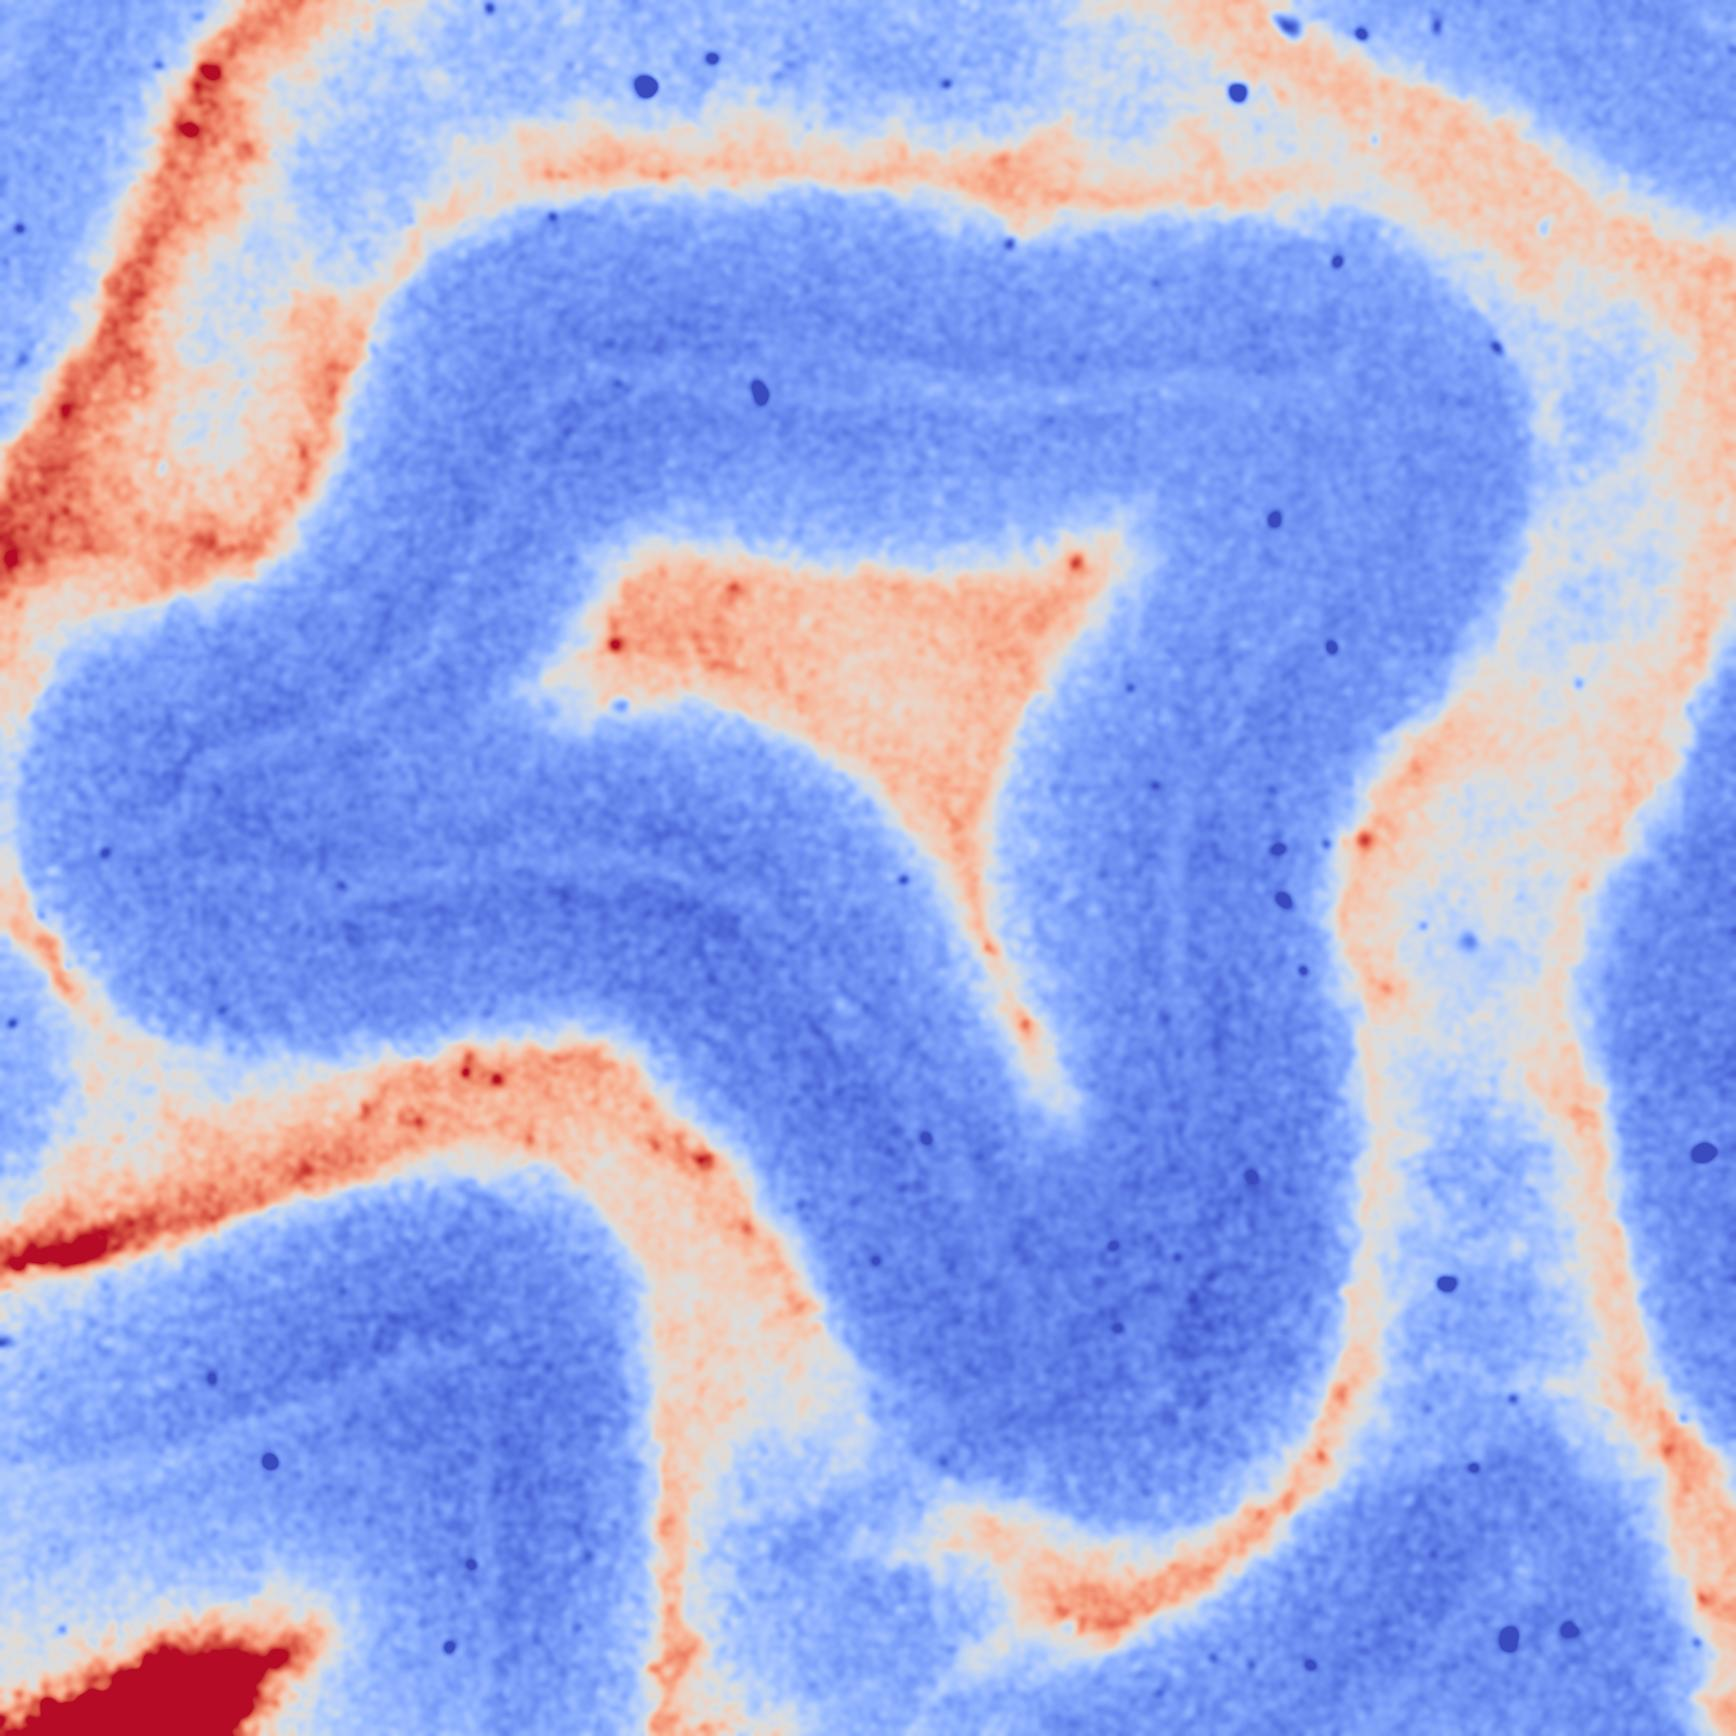
\includegraphics[width=0.75\textwidth]{plastic_confocal}};
		\draw[ultra thick] (a.south west) -- ++(0.41\textwidth,0) node[pos=0.5, above=0, font=\small] {\SI{500}{\micro\metre}};
\end{tikzpicture}
5\%
\end{block}
\begin{itemize}
\item Encore plus d'harmonique
\item Même longueur d'onde primaire
\item Plasticité
\end{itemize}
\end{columns}
\end{frame}

\begin{frame}{Diagramme de phase}
\begin{tikzpicture}
\begin{axis}[%
	name=phasediag,
	width=0.9\textwidth,
	height=0.6\textwidth,
	xmin=0,xmax=4.5,xlabel={\% caseinate}, xtick={1,2,3,4},
	ymin=0,ymax=5,ylabel={\% GDL},
	legend style={legend pos=north west,},
	xlabel near ticks,
	ylabel near ticks,
	]
\node at (axis cs:1,1) {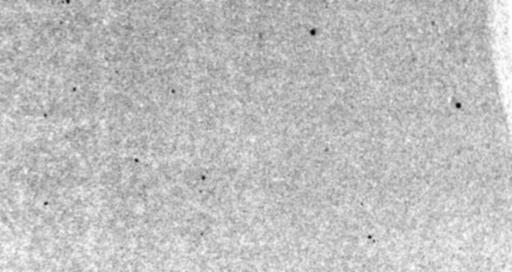
\includegraphics[width=0.15\textwidth]{cas1_GDL1.jpg}};
\node at (axis cs:2,1) {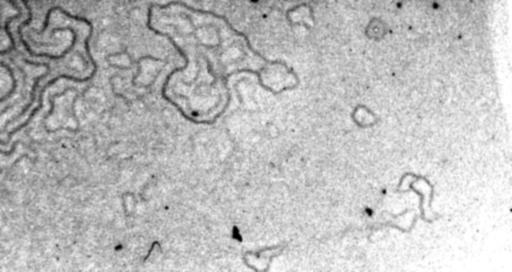
\includegraphics[width=0.15\textwidth]{cas2_GDL1.jpg}};
\node at (axis cs:2,2) {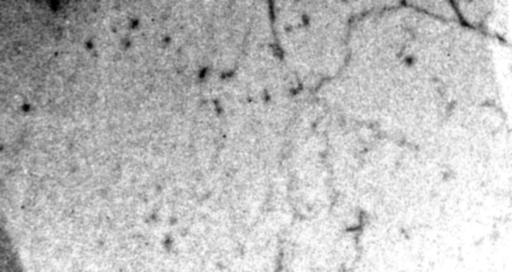
\includegraphics[width=0.15\textwidth]{cas2_GDL2.jpg}};
\node at (axis cs:3,1) {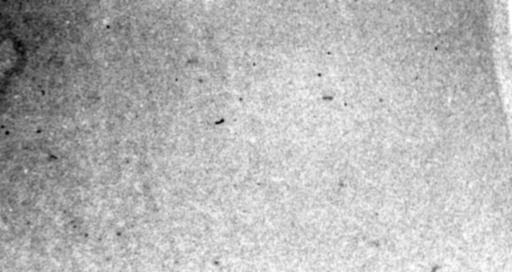
\includegraphics[width=0.15\textwidth]{cas3_GDL1.jpg}};
\node at (axis cs:3,2) {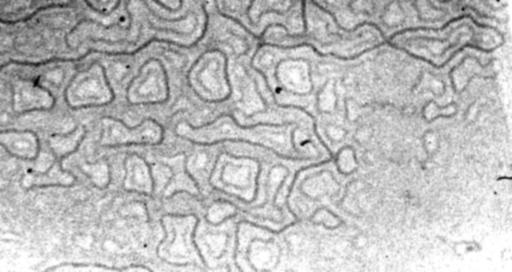
\includegraphics[width=0.15\textwidth]{cas3_GDL2.jpg}};
\node at (axis cs:3,3) {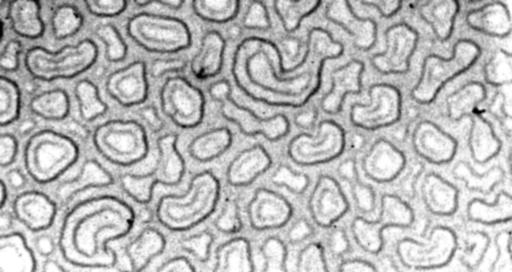
\includegraphics[width=0.15\textwidth]{cas3_GDL3.jpg}};
\node at (axis cs:4,1) {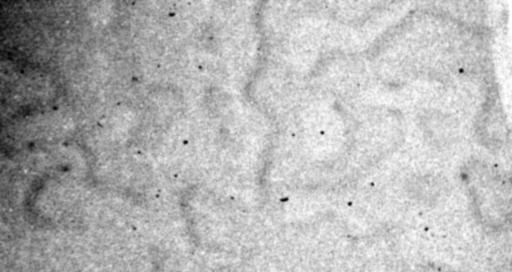
\includegraphics[width=0.15\textwidth]{cas4_GDL1.jpg}};
\node at (axis cs:4,2) {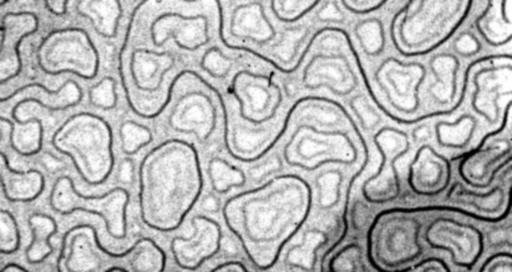
\includegraphics[width=0.15\textwidth]{cas4_GDL2.jpg}};
\node at (axis cs:4,3) {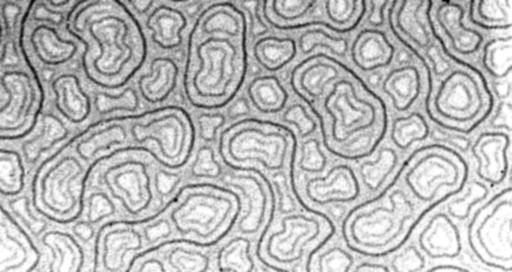
\includegraphics[width=0.15\textwidth]{cas4_GDL3.jpg}};
\node at (axis cs:4,4) {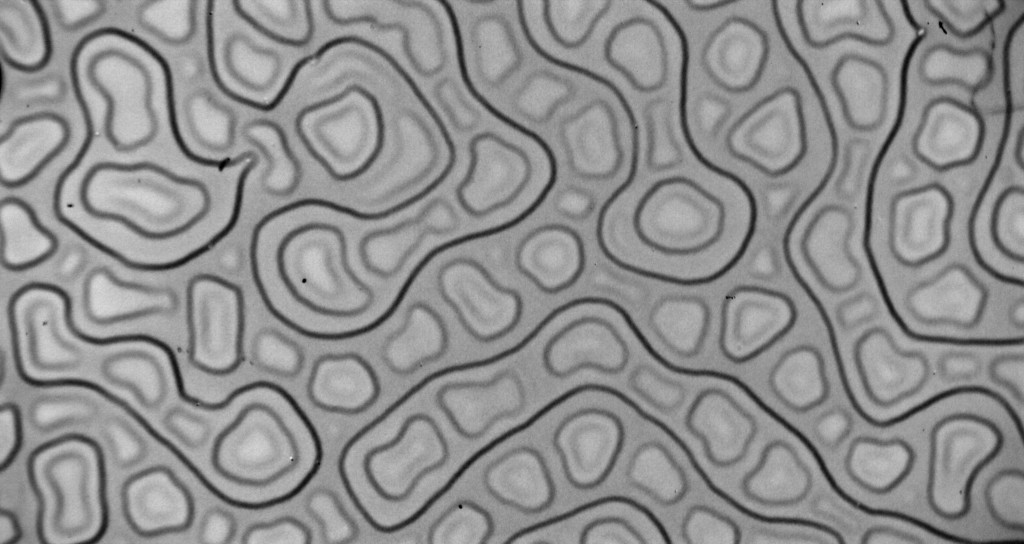
\includegraphics[width=0.15\textwidth]{pattern_100um.jpg}};
\addplot[no marks, Accent1] coordinates {(0,0) (5,5)} node[pos=0.05,above] {\SI{1}{\hour}};
\addplot[no marks, Main] coordinates {(0,0) (10,5)} node[pos=0.075] {\SI{2}{\hour}};
\addplot[no marks, Accent2] coordinates {(0,0) (8,2)} node[pos=0.2,below] {\SI{8}{\hour}};

\node at (axis cs:1,4) {$\lambda = \sqrt{hH} \left(\frac{E_f}{E_s}\right)^\frac{1}{6}$};

\end{axis}
\draw[->] ($(phasediag.north east)+(1em,0)$) -- ($(phasediag.south east)+(1em,0)$) node[midway,right,text width=0.1\textwidth] {\begin{align*}
\frac{G^{\prime}_\infty}{G^{\prime}_\text{max}}&\nearrow\\
\delta&\searrow
\end{align*}};
\draw[->] ($(phasediag.north west)+(0,1em)$) -- ($(phasediag.north east)+(0,1em)$) node[midway,above] {$G^{\prime}_\text{max}, E_f, h\nearrow$};
\end{tikzpicture}
\end{frame}

\end{document}